\documentclass[twocolumn]{article}

\usepackage{preprint}
\usepackage{graphicx}
\usepackage{tikz}
\usepackage{adjustbox}
\usepackage[most]{tcolorbox}
\usepackage{xcolor}
\usepackage{wrapfig}
\usepackage[hidelinks]{hyperref}

\title{Replicable experiments using OpenTTD}
\author{Michal Charemza}
\date{April 2023}

% From https://www.overleaf.com/latex/templates/sticky-notes/ftrvjddrmbwx
% Vebjørn S. Førde
% Creative Commons CC BY 4.0
% Yellow:
\definecolor{BgYellow}{HTML}{FFF59C}
\definecolor{FrameYellow}{HTML}{F7A600}
\newtcolorbox{YStkyNote}[1][]{%
    enhanced,
    before skip=2mm,after skip=2mm, 
    width=\columnwidth - 3mm, % width of the sticky note
    boxrule=0.2mm,
    colback=BgYellow, colframe=FrameYellow, % Colors
    attach boxed title to top left={xshift=0cm,yshift*=0mm-\tcboxedtitleheight},
    varwidth boxed title*=-3cm,
    % The titlebox:
    boxed title style={frame code={%
        \path[left color=FrameYellow,right color=FrameYellow,
        middle color=FrameYellow]
        ([xshift=-0mm]frame.north west) -- ([xshift=0mm]frame.north east)
        [rounded corners=0mm]-- ([xshift=0mm,yshift=0mm]frame.north east)
        -- (frame.south east) -- (frame.south west)
        -- ([xshift=0mm,yshift=0mm]frame.north west)
        [sharp corners]-- cycle;
        },interior engine=empty,
    },
    sharp corners,rounded corners=southeast,arc is angular,arc=3mm,
    % The "folded paper" in the bottom right corner:
    underlay={%
        \path[fill=BgYellow!80!black] ([yshift=3mm]interior.south east)--++(-0.4,-0.1)--++(0.1,-0.2);
        \path[draw=FrameYellow,shorten <=-0.05mm,shorten >=-0.05mm,color=FrameYellow] ([yshift=3mm]interior.south east)--++(-0.4,-0.1)--++(0.1,-0.2);
        },
    drop fuzzy shadow, % Shadow
    fonttitle=\bfseries, 
    title={#1}
}

\begin{document}

\twocolumn[
  \begin{@twocolumnfalse}
  
    \maketitle

    \begin{abstract}
        OpenTTD is an open source real time strategy (RTS) business simulation game based on the 1994 game Transport Tycoon Deluxe. In spite of being designed as a recreational game, OpenTTD has been the focus of a number of academic studies. However, these studies have problems regarding the replicability of their experiments. This paper summarises the problems, and suggests patterns of usage of OpenTTD to avoid these problems in future research.
    \end{abstract}
\vspace{0.35cm}

  \end{@twocolumnfalse}
]

\section{Introduction}

OpenTTD \cite{openttd} is an open source real time strategy (RTS) simulation game. The aim of the game is to successfully run a business by constructing networks of roads, railways, airports and ports, along with their respective vehicles, trains, planes and ships, in order to transport people and goods in exchange for money. OpenTTD is played on a simulated landscape as can be seen in Figure \ref{fig:openttd}.

\begin{figure}[h]
\centering
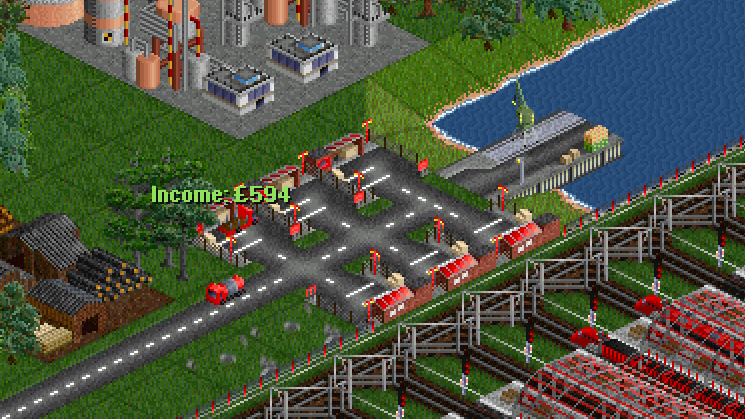
\includegraphics[width=\columnwidth]{assets/openttd-screenshot.png}
\caption{A small section of an OpenTTD (version 12.2) game at the moment when income is received for delivering goods by road. Also shown is part of a railway network, a port for ships, an oil refinery, and a sawmill.}
\label{fig:openttd}
\end{figure}

OpenTTD was created as a game for recreation. However, it is remarkably flexible: it has been successfully used as a tool to research artificial intelligence (AI) and machine learning (ML) algorithms \cite{wisniewski2011artificial, rios2009trains, bijlsma2014evolving}, scalability and mobile applications \cite{jiang2018mirroring}, and as a teaching aid \cite{HansenMuprhie2018}. Using it a a tool for research is the focus of this paper, and specifically its features for replicable research.

\section{Repeatability, Replicatability, \& Reproducibility }
\begin{YStkyNote}
Explain the differences
\end{YStkyNote}

Is this, methods and results \cite{plesser_reproducibility_2018}

\section{Review of research using OpenTTD}

\begin{YStkyNote}
Give specific examples of the research and issues in research
\end{YStkyNote}

\section{Review of OpenTTD command line options and configuration}
OpenTTD as of version 13.4 has over X command line options and Y configuration options that allow the player to customise how it behaves when playing. The ones that are particularly applicable are reviewed below

\subsection{Command line options}

\begin{description}
\item[-G \textless seed\textgreater] Allows the specification of the seed that initialises the random number generator that controls the pseudo random aspects of the game. For example, OpenTTD can auto generate landscapes. With the same seed (along with other configuration) one generation will be the same as the next
\item[-g] Starts a game immediately, rather than requiring the user to click through a introductory menu 
\item[-vnull:ticks=\textless number of ticks\textgreater] Puts the same into a "null" video mode that does not display the playing area on screen, and exits the game after a set number of \emph{ticks}. A tick is equal to approximately 1/Y of a day in game time.
\end{description}

\subsection{Configuration options}

\begin{description}
\item[{fast\_forward\_speed\_limit} = \textless limit\textgreater] Limits the ticks per second the limit, which has a hard coded maximum in the game of 50000

\item[{[ai\_players]}] Allows the specification of which player are human and which are AI, and when they start playing.

\item[autosave = monthly|daily|other CHECK]

\item[keep\_all\_autosave]  A boolean value that allows all autosaves to be kept for further analysis
\end{description}

\section{Extracting data from OpenTTD}

OpenTTD does saves its data in a custom binary format. OpenTTD offers an extremely basic tool for extracting some data from this format, but it only shows X and Y.

Extracting data from this format into a structure that is ready to be analysed.

\section{Example results using these patterns}




\section{Possible extensions to OpenTTD}

Disable the max fast forward speed limit

Maximum number of autosaves

\begin{YStkyNote}
Suggest extensions that would address the issues of the research
\end{YStkyNote}

There are limited ways in which to extract data from the game.
Fast forward has a limit.
Can I be a spectator?

\section{Research vs. recreation}

\begin{YStkyNote}
OpenTTD is a game, and not for research. Is there a tension? Could it be for both?
\end{YStkyNote}

\section{Conclusion}

\begin{YStkyNote}
Briefly repeat the main points above
\end{YStkyNote}

\normalsize
\bibliographystyle{unsrt}
\bibliography{main}

\end{document}
